\documentclass{standalone}
\usepackage{tikz}
\usetikzlibrary{shapes,fit}
\usepackage{arydshln}
\usepackage{systems}
\begin{document}
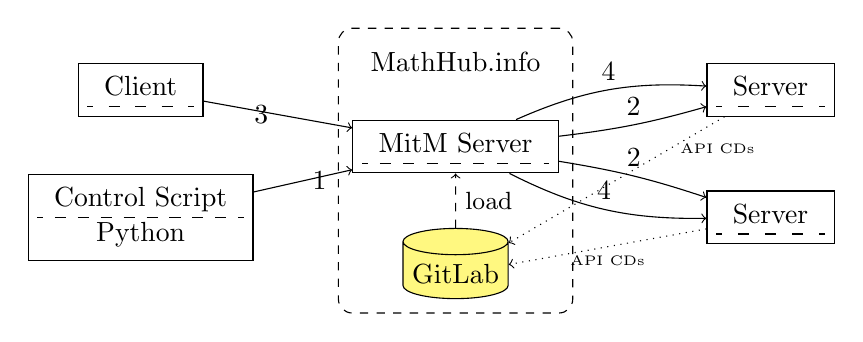
\begin{tikzpicture}[xscale=2, yscale=1.8]\normalsize
   \tikzstyle{database} = [cylinder,cylinder uses custom fill,
      cylinder body fill=yellow!50,cylinder end fill=yellow!50,
      shape border rotate=90, 
      aspect=0.25,draw]
  \node (mh) at (2,1.4) {MathHub.info};
  \node[draw,database] (gl) at (2,-.1) {GitLab};
  \node[draw] (m) at (2,.8) {
    \begin{tabular}{c}
      MitM Server\\\hdashline \MMT
    \end{tabular}
  };
  \node[draw,dashed,rounded corners=5pt,fit=(mh) (m) (gl),inner sep=5pt] {}; 

  \node[draw] (g) at (4,1.2) {
    \begin{tabular}{c}
      \GAP Server \\\hdashline \GAP
    \end{tabular}
  };
  \node[draw] (s) at (4,.3) {
    \begin{tabular}{c}
     \Singular Server\\\hdashline \Singular
    \end{tabular}
  };
  \node[draw] (p) at (0,1.2) {
    \begin{tabular}{c}
      \Sage Client\\\hdashline \Sage
    \end{tabular}
  };
  \node[draw] (c) at (0,.3) {
    \begin{tabular}{c}
      Control Script\\\hdashline Python
    \end{tabular}
    };
    \draw[dashed,->] (gl) -- node[right] {\small load} (m);
    \draw[dotted,->] (g) -- node[right,near start] {\tiny API CDs} (gl); 
    \draw[dotted,->] (s) -- node[below] {\tiny API CDs} (gl); 
    \draw[->] (c) to node[right] {1} (m);
    \draw[->] (m) to[bend left=5] node[above] {2} (s);
    \draw[->] (m) to[bend right=5] node[above] {2} (g);
    \draw[->] (p) to node[left] {3} (m);
    \draw[->] (m) to[bend right=15] node[above] {4} (s);
    \draw[->] (m) to[bend left=15] node[above] {4} (g);
  \end{tikzpicture}
\end{document}
% LocalWords:  tikzpicture xscale yscale Singuler

%%% Local Variables:
%%% mode: latex
%%% TeX-master: t
%%% End:
